\documentclass[11pt]{article}
\usepackage[utf8]{inputenc} % Para caracteres en espa�ol
\usepackage{amsmath,amsthm,amsfonts,amssymb,amscd}
\usepackage{multirow,booktabs}
\usepackage[table]{xcolor}
\usepackage{fullpage}
\usepackage{lastpage}
\usepackage{enumitem}
\usepackage{multicol}
\usepackage{fancyhdr}
\usepackage{mathrsfs}
\usepackage{wrapfig}
\usepackage[final]{pdfpages}
\usepackage{setspace}
\usepackage{esvect}
\usepackage{calc}
\usepackage{multicol}
\usepackage{cancel}
\usepackage{graphicx}
\graphicspath{ {pictures/} }
\usepackage[retainorgcmds]{IEEEtrantools}
\usepackage[margin=3cm]{geometry}
\usepackage{amsmath}
\newlength{\tabcont}
\setlength{\parindent}{0.0in}
\setlength{\parskip}{0.05in}
\usepackage{empheq}
\usepackage{framed}
%\usepackage{newtxmath}
\usepackage{euscript}
\DeclareMathAlphabet{\mathpzc}{T1}{pzc}{m}{it}
\usepackage[most]{tcolorbox}
\usepackage{xcolor}
\colorlet{shadecolor}{orange!15}
\parindent 0in
\parskip 12pt
\geometry{margin=1in, headsep=0.25in}
\theoremstyle{definition}
\newtheorem{defn}{Definition}
\newtheorem{reg}{Rule}
\newtheorem{exer}{Exercise}
\newtheorem{note}{Note}
\newcommand{\volume}{{\ooalign{\hfil$V$\hfil\cr\kern0.08em--\hfil\cr}}}
\newcommand{\parr}{\mathbin{\|}} % Parralel Symbol
\begin{document}
\setcounter{section}{2}%Section we want -1
\setcounter{page}{27} %Page we want
\setcounter{equation}{36}%Equation we want -1
\def\thepart{\arabic{part}}
\setcounter{part}{8}
\numberwithin{equation}{part}

 \pagestyle{fancy}
\fancyhf{}
\rhead{Section 8:  Electromagnetic Propulsion - Pulse Forming Networks}
\rfoot{Page \thepage}
\thispagestyle{empty}

\begin{center}
{\LARGE \bf Section 8:  Electromagnetic Propulsion}\\
{\large AE435}\\
Spring 2018
\end{center}
\vspace{5mm}
\section{Pulse Forming Networks}
\vspace{25mm}
\tableofcontents
\newpage
Where to get large (10's of kA) of current? We want to drive a lot of current through these electric propulsion systems. All of these EP systems have a power processing unit that provides the power necessary for the system to run, usually a Pulse Forming Network.
 
\subsection{Basic circuit theory:}
\subsubsection{LC Circuit:}  
Close switch, get sinusoidal oscillation of current. Capacitor is charged to a voltage Vo. You close the switch, the charge stored in the capacitor goes from being stored electrical energy in the capacitor to stored magnetic field energy in the inductor and is oscillated between these two forms indefinitely.

\begin{center}
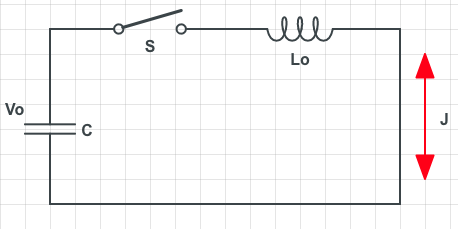
\includegraphics[scale=0.70]{LC.png} 

\vfill
\textbf{Figure 2: Current V. Time}
\end{center}
\begin{equation*}
\begin{aligned}
J = J_o \, \sin(\omega \, t) \qquad \qquad 
\omega = \sqrt{\frac{1}{L_o \, C}}
\end{aligned}
\end{equation*}
 \newpage
\subsubsection{LRC Circuit:}  Energy is now dissipated in load, R, which can have a Z component (reactive component).  Wave form depends on value of R.
 \begin{center}
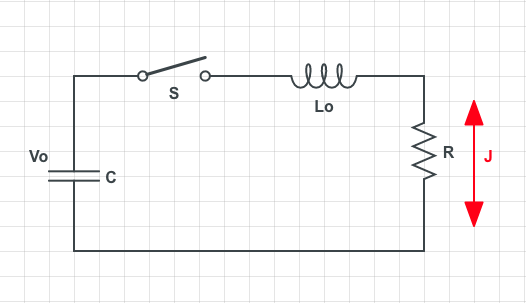
\includegraphics[scale=0.7]{LCR.png} \\
\vfill
\begin{equation*}
\begin{aligned}
R<2 \, \sqrt{\frac{L_o}{C}} \qquad \qquad \qquad \qquad  \qquad \qquad  \qquad \qquad  \qquad \qquad R = 2 \, \sqrt{\frac{L_o}{C}}
\end{aligned}
\end{equation*}
\textbf{Figure 3: Small R - Underdamped} \hspace{30mm}\textbf{Figure 4: Critically Damped}

\begin{equation*}
\begin{aligned}
\textbf{Total Dissipated Energy:} = \frac{1}{2} \, C \, V_o^2
\end{aligned}
\end{equation*}
 \end{center}
 
Critically damped is good because current does not reverse, but it does not give a constant current, $J  \neq  const$. Ideally, we want something resembling a square wave where the current goes from on to off without having to ramp-up/down to its value. Solution is to replace $L_o$ and $C$, with a distributed $L'$ and $C'$ to give us a fairly constant current.
 \newpage
\begin{framed}
\textbf{Example:} A Coaxial cable has a distributed capacitance and inductance.
 
 \begin{center}
 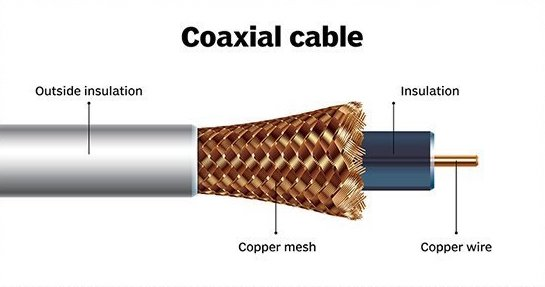
\includegraphics[scale=0.6]{coaxcable.jpg}
 
 \begin{equation*}
\begin{aligned}
L = L' \, l \qquad C = C' \, l \qquad \text{Impedance} = \sqrt{\frac{L'}{C'}} = 50 \Omega
\end{aligned}
\end{equation*}
 \end{center}
 Where
  \begin{equation*}
\begin{aligned}
L &= \text{Inductance [H]}\\
L' &= \text{Inductance Per Unit Length [H/m]}\\
C &= \text{Capacitance [F]}\\
C' &= \text{Capacitance Per Unit Length [F/m]}\\
l &= \text{Total Length [m]}\\
\end{aligned}
\end{equation*}

$50 \Omega $ is always used because it is the impedance for most data acquisition instruments.

As such...

\textbf{Total Dissipated Energy:}
\begin{equation*}
\begin{aligned}
 E_o &= \frac{1}{2} \, C' \, l \, V_o^2
\end{aligned}
\end{equation*}

\textbf{Pulse Duration:} 
\begin{equation*}
\begin{aligned}
t_p &= 2 \, l \, \sqrt{L' \, C'}
\end{aligned}
\end{equation*}
 
 
Pulse velocity $\sim 1 \, ft/sec$ (speed of light), so for a $5 \, \mu s$ pulse $\rightarrow 5000 \, ft=1 \, mi$ of cable required which is Prohibitively massive!

Instead, use lumped transmission line or \textbf{Pulse Forming Network}. Must always match \textbf{impedance of PFN to thruster!}
 \end{framed}
 \newpage
\subsection{Pulse forming network}
 
   \begin{center}
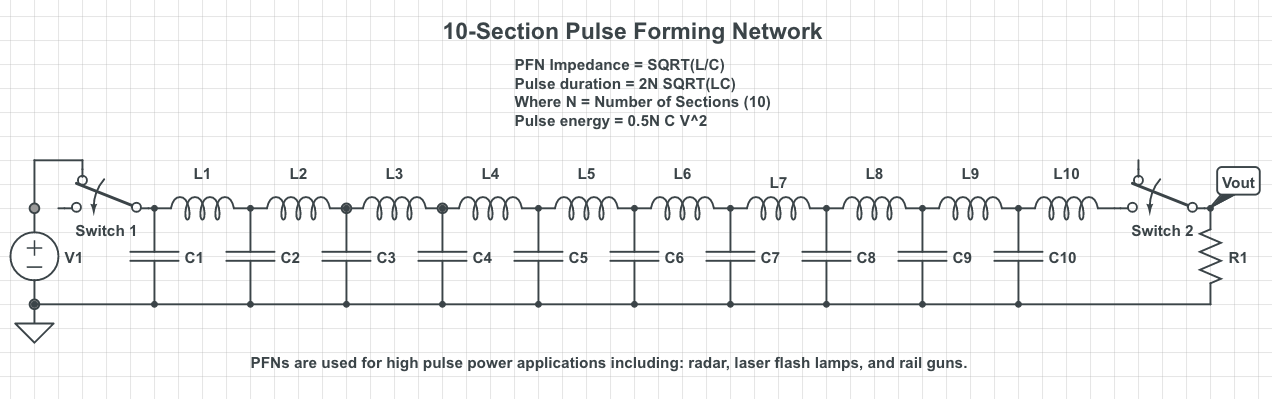
\includegraphics[scale=0.4]{PFN.png} 
\end{center}

Shown above is a 10 section PFN. Typically N-section/element PFN.  Equivalent to coax cable as $N \rightarrow \infty$

For
 \begin{equation*}
\begin{aligned}
Z = \sqrt{\frac{L}{C}} \rightarrow \text{Matched Pulse Forming Network} \\ \\
\end{aligned}
\end{equation*}
 \begin{equation*}
\begin{aligned}
t_p = 2 \, N \, \sqrt{L \, C} \qquad \qquad 
J = \frac{V_o}{2 \, Z}
\end{aligned}
\end{equation*}

 For a "good" square pulse, $N \ge 5$. In other words, we need a 5 section pulse forming network to get a relatively square wave current profile as desired.
 \vfill
 \newpage
 For MPD need high current, so want small Z.  
 \begin{framed}
 \textbf{Example: } Consider a 10-Section Pulse Forming network with an input voltage, $V_o = 200 \, V$, and current $J = 20 \, kA$. This implies an impedance of, $Z = 5 \, m\Omega$. The capacitors on the PFN are $C = 0.001 \, F = 1 \, mF$. Find the Pulse Duration, Power per Pulse, Energy, Average Power, and the Duty Cycle of this PFN.
 
 If $Z = 5 \, m\Omega$...
 
    \begin{equation*}
\begin{aligned}
L = C \, Z^2 \rightarrow C\,Z = 5 \, [\mu \, sec] \rightarrow L = 25 \, [n \, H]
\end{aligned}
\end{equation*}
 
 If $N=10$...
 
   \begin{equation*}
\begin{aligned}
t_p = 2 \, N \, \sqrt{L \, C} = 2 \cdot 10 \, \sqrt{L \, C} = 100 \, [\mu s] \\ \\
P = J^2 \, Z = 2 \, [MW/\text{pulse}] \\ \\
E = P \cdot t_p = 200 \, [J] \\ \\
\end{aligned}
\end{equation*}
\begin{center}
\begin{tabular}{ c c c }
\textbf{If our PFN at 1 $Hz$} &\quad & \textbf{If our PFN at 100 $Hz$} \\ [1em]
$P_{avg} = E \times \text{pulse rate} = 200 \, [W]$ &\quad & $P_{avg} = E \times \text{pulse rate} = 20 \, [kW]$
\end{tabular}
\end{center}
\end{framed}
\newpage
\subsection{Problems with Pulse Forming Networks:}
\begin{enumerate}
\item We find for the MPD           $Z \sim \frac{200 \,  [V]}{20,000 \, [A]} = 10 \, [m \Omega]$                         so                       needs to be $10 \, [m \Omega]$ not $5 \, [m \Omega]$.    Need to match or will get lossy reflections, other reactive elements (C or L) required.
\item Switching, need reliable, 1 Hz, 20 kA switch at 200 V.  With a lifetime of $10^8 - 10^{12}$ pulses ($\sim$3 yrs).  Very difficult!
\begin{enumerate}
\item Mechanical too slow
\item Krytron vacuum tube - space charge limited
\item $H_2$ thyratron tube - high voltage, but not high current
\item Hg ignitron - high currrent, but Hg pool, not good in zero-g
\item Vacuum gap - short life, erodes electrodes
\item Solid state switches - low current and slow, SCRs
\end{enumerate}
Many of these high current switches originally developed by fusion community in 1950-1960's.  Probably the most promising is the SCR (silicon controlled rectifier), but long life is still a challenge.  This is a major issue for MPD and other high current EM thrusters.
\item Feed system.  Duty cycle of $10^{-4}$ can't run mass flow rate continuously!  Need fast valve with $10^8$ cycle life.  Fastest is$ \sim$1 msec.  Could extend $t_p\sim$1000sec.  But now the PFN get heavy... need more elements or larger LC...

Some research has focused on liquid metals as a means to remove the feed system requirement.  Input mass flow rate due to evaporation of the cathode due to the discharge itself.  E.g., lithium, bismuth, gallium propellant MPDs.
 \end{enumerate}
 
 
 


\end{document}